\documentclass[]{tufte-handout}

% ams
\usepackage{amssymb,amsmath}

\usepackage{ifxetex,ifluatex}
\usepackage{fixltx2e} % provides \textsubscript
\ifnum 0\ifxetex 1\fi\ifluatex 1\fi=0 % if pdftex
  \usepackage[T1]{fontenc}
  \usepackage[utf8]{inputenc}
\else % if luatex or xelatex
  \makeatletter
  \@ifpackageloaded{fontspec}{}{\usepackage{fontspec}}
  \makeatother
  \defaultfontfeatures{Ligatures=TeX,Scale=MatchLowercase}
  \makeatletter
  \@ifpackageloaded{soul}{
     \renewcommand\allcapsspacing[1]{{\addfontfeature{LetterSpace=15}#1}}
     \renewcommand\smallcapsspacing[1]{{\addfontfeature{LetterSpace=10}#1}}
   }{}
  \makeatother
\fi

% graphix
\usepackage{graphicx}
\setkeys{Gin}{width=\linewidth,totalheight=\textheight,keepaspectratio}

% booktabs
\usepackage{booktabs}

% url
\usepackage{url}

% hyperref
\usepackage{hyperref}

% units.
\usepackage{units}


\setcounter{secnumdepth}{-1}

% citations

% pandoc syntax highlighting
\usepackage{color}
\usepackage{fancyvrb}
\newcommand{\VerbBar}{|}
\newcommand{\VERB}{\Verb[commandchars=\\\{\}]}
\DefineVerbatimEnvironment{Highlighting}{Verbatim}{commandchars=\\\{\}}
% Add ',fontsize=\small' for more characters per line
\newenvironment{Shaded}{}{}
\newcommand{\KeywordTok}[1]{\textcolor[rgb]{0.00,0.44,0.13}{\textbf{{#1}}}}
\newcommand{\DataTypeTok}[1]{\textcolor[rgb]{0.56,0.13,0.00}{{#1}}}
\newcommand{\DecValTok}[1]{\textcolor[rgb]{0.25,0.63,0.44}{{#1}}}
\newcommand{\BaseNTok}[1]{\textcolor[rgb]{0.25,0.63,0.44}{{#1}}}
\newcommand{\FloatTok}[1]{\textcolor[rgb]{0.25,0.63,0.44}{{#1}}}
\newcommand{\ConstantTok}[1]{\textcolor[rgb]{0.53,0.00,0.00}{{#1}}}
\newcommand{\CharTok}[1]{\textcolor[rgb]{0.25,0.44,0.63}{{#1}}}
\newcommand{\SpecialCharTok}[1]{\textcolor[rgb]{0.25,0.44,0.63}{{#1}}}
\newcommand{\StringTok}[1]{\textcolor[rgb]{0.25,0.44,0.63}{{#1}}}
\newcommand{\VerbatimStringTok}[1]{\textcolor[rgb]{0.25,0.44,0.63}{{#1}}}
\newcommand{\SpecialStringTok}[1]{\textcolor[rgb]{0.73,0.40,0.53}{{#1}}}
\newcommand{\ImportTok}[1]{{#1}}
\newcommand{\CommentTok}[1]{\textcolor[rgb]{0.38,0.63,0.69}{\textit{{#1}}}}
\newcommand{\DocumentationTok}[1]{\textcolor[rgb]{0.73,0.13,0.13}{\textit{{#1}}}}
\newcommand{\AnnotationTok}[1]{\textcolor[rgb]{0.38,0.63,0.69}{\textbf{\textit{{#1}}}}}
\newcommand{\CommentVarTok}[1]{\textcolor[rgb]{0.38,0.63,0.69}{\textbf{\textit{{#1}}}}}
\newcommand{\OtherTok}[1]{\textcolor[rgb]{0.00,0.44,0.13}{{#1}}}
\newcommand{\FunctionTok}[1]{\textcolor[rgb]{0.02,0.16,0.49}{{#1}}}
\newcommand{\VariableTok}[1]{\textcolor[rgb]{0.10,0.09,0.49}{{#1}}}
\newcommand{\ControlFlowTok}[1]{\textcolor[rgb]{0.00,0.44,0.13}{\textbf{{#1}}}}
\newcommand{\OperatorTok}[1]{\textcolor[rgb]{0.40,0.40,0.40}{{#1}}}
\newcommand{\BuiltInTok}[1]{{#1}}
\newcommand{\ExtensionTok}[1]{{#1}}
\newcommand{\PreprocessorTok}[1]{\textcolor[rgb]{0.74,0.48,0.00}{{#1}}}
\newcommand{\AttributeTok}[1]{\textcolor[rgb]{0.49,0.56,0.16}{{#1}}}
\newcommand{\RegionMarkerTok}[1]{{#1}}
\newcommand{\InformationTok}[1]{\textcolor[rgb]{0.38,0.63,0.69}{\textbf{\textit{{#1}}}}}
\newcommand{\WarningTok}[1]{\textcolor[rgb]{0.38,0.63,0.69}{\textbf{\textit{{#1}}}}}
\newcommand{\AlertTok}[1]{\textcolor[rgb]{1.00,0.00,0.00}{\textbf{{#1}}}}
\newcommand{\ErrorTok}[1]{\textcolor[rgb]{1.00,0.00,0.00}{\textbf{{#1}}}}
\newcommand{\NormalTok}[1]{{#1}}

% longtable

% multiplecol
\usepackage{multicol}

% strikeout
\usepackage[normalem]{ulem}

% morefloats
\usepackage{morefloats}


% tightlist macro required by pandoc >= 1.14
\providecommand{\tightlist}{%
  \setlength{\itemsep}{0pt}\setlength{\parskip}{0pt}}

% title / author / date
\title{Unsupervised Genetics}
\author{Data Computing}
\date{Computing project}


\begin{document}

\maketitle




\begin{small}

There are many different kinds of cancer, often given the name of the tissue in which they originate: lung cancer, ovarian cancer, prostate cancer, and so on.

In this exercise, you are going to look for possible relationships among different cancer types.  The basis for this will be the data in \texttt{NCI60}, which records the level of gene expression indicated by each of 41,078 probes against each of 60 different cell lines collected from different people with different kinds of cancer.


Looking at so many probes is a kind of shotgun approach enabled by 
{\em microarray} chips.  It's assumed that only a few genes might be involved in any given type of cancer; by looking at the expression of many genes, it's hoped to be able to identify those few.
\end{small}

\section{Clustering the cancer types}\label{clustering-the-cancer-types}

\begin{small}
The point of clustering is to identify pairs or sets of cases that are similar.  In *hierarchical clustering*, the pairs or sets are themselves grouped together in terms of similarity.  The result is a kind of tree, a *dendrogram*, that shows which cases and sets of cases are similar.

\begin{marginfigure}
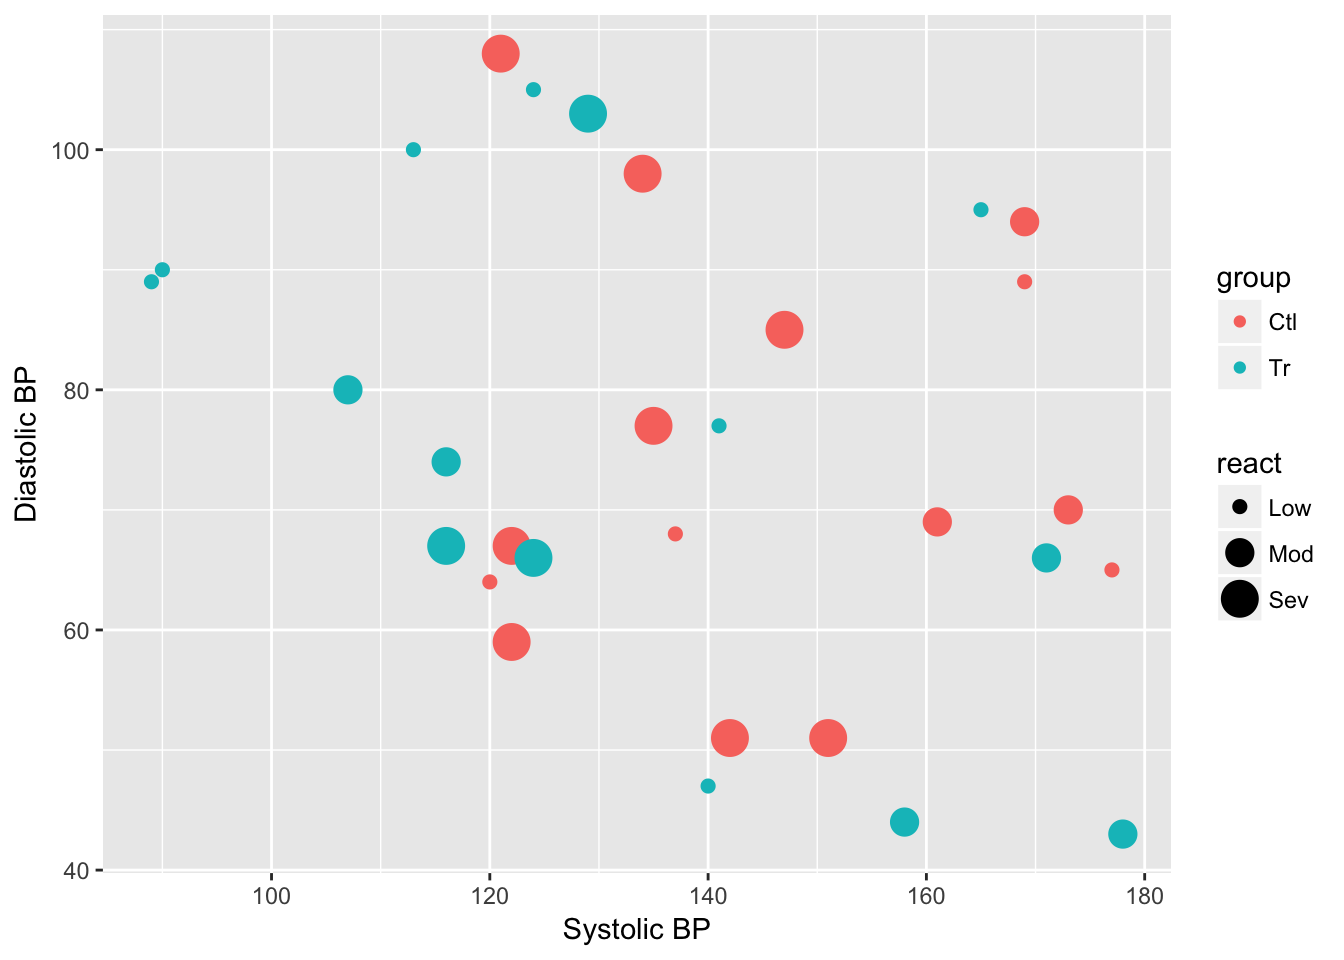
\includegraphics{863-UnsupervisedGenetics_files/figure-latex/unnamed-chunk-2-1} \end{marginfigure}

As an example, here is a dendrogram constructed for the different cars in `mtcars`.  There are two major groups of cars.  From the base of the tree, two branches identify two major groups of cars.  Each of those groups is subdivided, with the process repeating until reaching a *leaf*: an individual case.  The level of the horizontal line connecting two sub-branches indicates the distance between those sub-branches.  For example, the Honda Civic, Toyota Corolla, and Fiat 128 are quite similar.

Glyph-ready data for constructing a dendrogram is in the usual tidy form, with the cases being the objects to cluster and the variables being the means to judge similarity between cases. The `mtcars` data table is already in glyph-ready form; take a look! Note that the identifiers for the object, e.g. "Datsun 710," are not stored in a variable but in the *row names* of the data table.

\end{small}

\marginnote[ -1cm ]{ \noindent{\begin{tabular}{rrrrr}
  \toprule
mpg & cyl & disp & hp & drat \\ 
  \midrule
21.00 &   6 & 160.00 & 110 & 3.90 \\ 
  21.00 &   6 & 160.00 & 110 & 3.90 \\ 
  22.80 &   4 & 108.00 &  93 & 3.85 \\ 
  21.40 &   6 & 258.00 & 110 & 3.08 \\ 
  18.70 &   8 & 360.00 & 175 & 3.15 \\ 
   \multicolumn{5}{c}{... {\em and so on for 32 rows}}\\ \bottomrule
\end{tabular}
}
\smallskip
Table 1. \texttt{mtcars}
\vspace*{2pt}

 }

The process is as follows:

\enlargethispage{1.5in}

\begin{enumerate}
\def\labelenumi{\arabic{enumi}.}
\item
  Find the distances from each case to every other case. The
  \texttt{dist()} function accomplishes this.

\begin{Shaded}
\begin{Highlighting}[]
\NormalTok{Dists <-}\StringTok{ }\KeywordTok{dist}\NormalTok{(mtcars)}
\end{Highlighting}
\end{Shaded}

  \vspace*{-.2in}
\item
  Apply the clustering algorithm to make the dendrogram.

\begin{Shaded}
\begin{Highlighting}[]
\NormalTok{Dendrogram <-}\StringTok{ }\KeywordTok{hclust}\NormalTok{(Dists)}
\NormalTok{ddata <-}\StringTok{ }\KeywordTok{dendro_data}\NormalTok{(Dendrogram)}
\end{Highlighting}
\end{Shaded}

  \vspace*{-.2in}
\item
  Visualize the dendrogram

\begin{Shaded}
\begin{Highlighting}[]
\KeywordTok{ggdendrogram}\NormalTok{(Dendrogram, }\DataTypeTok{rotate =} \OtherTok{TRUE}\NormalTok{) +}\StringTok{ }\KeywordTok{geom_text}\NormalTok{(}\DataTypeTok{data =} \NormalTok{ddata$labels, }
    \KeywordTok{aes}\NormalTok{(}\DataTypeTok{x =} \NormalTok{x, }\DataTypeTok{y =} \NormalTok{y, }\DataTypeTok{label =} \NormalTok{label), }\DataTypeTok{vjust =} \DecValTok{0}\NormalTok{)}
\end{Highlighting}
\end{Shaded}
\end{enumerate}

\section{Wrangling the genetics data}\label{wrangling-the-genetics-data}

The \texttt{NCI60} are not yet in a form suitable for clustering. There
are several shortcomings.

\begin{enumerate}
\def\labelenumi{\arabic{enumi}.}
\tightlist
\item
  The objects to be clustered --- cell lines --- are represented as
  variables instead of cases.
\item
  There are far too many probes to be able to identify ``similarity'' in
  a meaningful way. Recall that most of the probes are irrelevant.
\item
  The identifiers are not stored as the row names.
\end{enumerate}

To start, put the data in a narrow form, like Table 2.

\marginnote[ -2.5cm ]{ \noindent{\begin{tabular}{llr}
  \toprule
Probe & cellLine & expression \\ 
  \midrule
3.8-1 & BR.BT\_549 & -7.37 \\ 
  3.8-1 & BR.HS578T & -7.30 \\ 
  3.8-1 & BR.MCF7 & -7.45 \\ 
  3.8-1 & BR.MDA\_MB\_231 & -7.51 \\ 
  3.8-1 & BR.T47D & -7.74 \\ 
   \multicolumn{3}{c}{... {\em and so on for 1,940,640 rows}}\\ \bottomrule
\end{tabular}
}
\smallskip
Table 2. \texttt{NCI60} gathered into a narrow form. There is a row for each probe at each of the 60 cell lines.
\vspace*{2pt}

 }

It happens that the same probe can appear multiple times on the gene
chip. Combine all such repeats by grouping by \texttt{Probe} and
\texttt{cellLine} and summarizing each group with
\texttt{expression\ =\ mean(expression)}. Then use \texttt{ungroup()} on
the result.\footnote{When you group on more than one variable,
  \texttt{summarise()} leaves the result partially grouped. This can
  interfere with later operations.}

In the narrow form, there's a simple way to pull out probes that might
be of relevance to distinguishing among the different kinds of cancer.
Presumably, for a relevant probe the expression will vary a lot among
the cancer types. A very simple indicator of this is the \emph{standard
deviation} of each probe's expression. You can calculate this by
grouping over \texttt{Probe} and summarising with
\texttt{spread\ =\ sd(expression)}.

\begin{marginfigure}
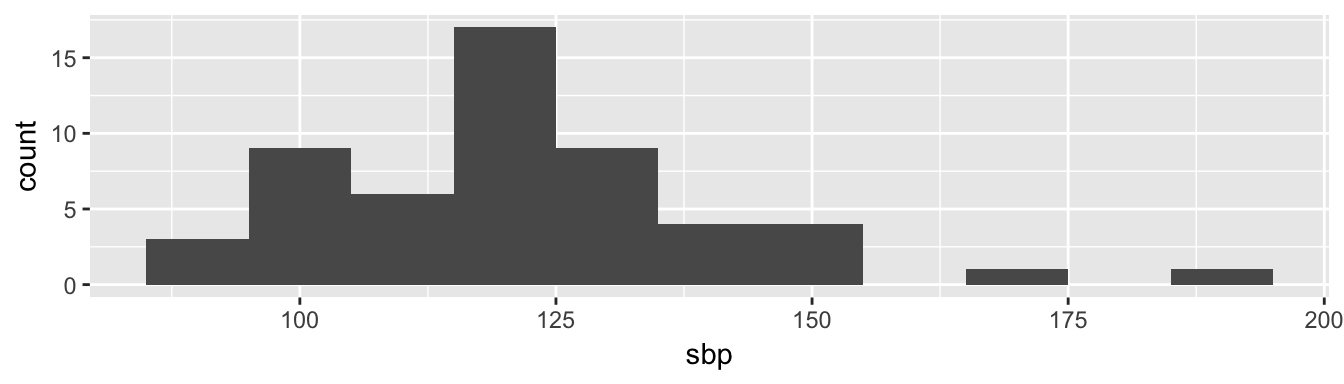
\includegraphics{863-UnsupervisedGenetics_files/figure-latex/unnamed-chunk-9-1} \caption[The spread of expression of probes across cell lines ordered from biggest to smallest for the leading 500 probes]{The spread of expression of probes across cell lines ordered from biggest to smallest for the leading 500 probes. For comparison, the red line shows the spread under the Null Hypothesis assumption that there is no relationship between probe and cell line.}\label{fig:unnamed-chunk-9}
\end{marginfigure}

Identify a threshold for \texttt{spread} that identifies potential
candidates for differential expression across cell lines and filter to
keep only the probes above that threshold.

Wrangle the result into a wide format with the variables being the
probes and the cases being the cell lines.

\enlargethispage{1.5in}

Cluster those cases and display your result. (You'll have to select out
the \texttt{cellLine} variable in the data table you hand to
\texttt{dist()}. The \texttt{dist()} function doesn't work with names
like those in \texttt{cellLine}.)

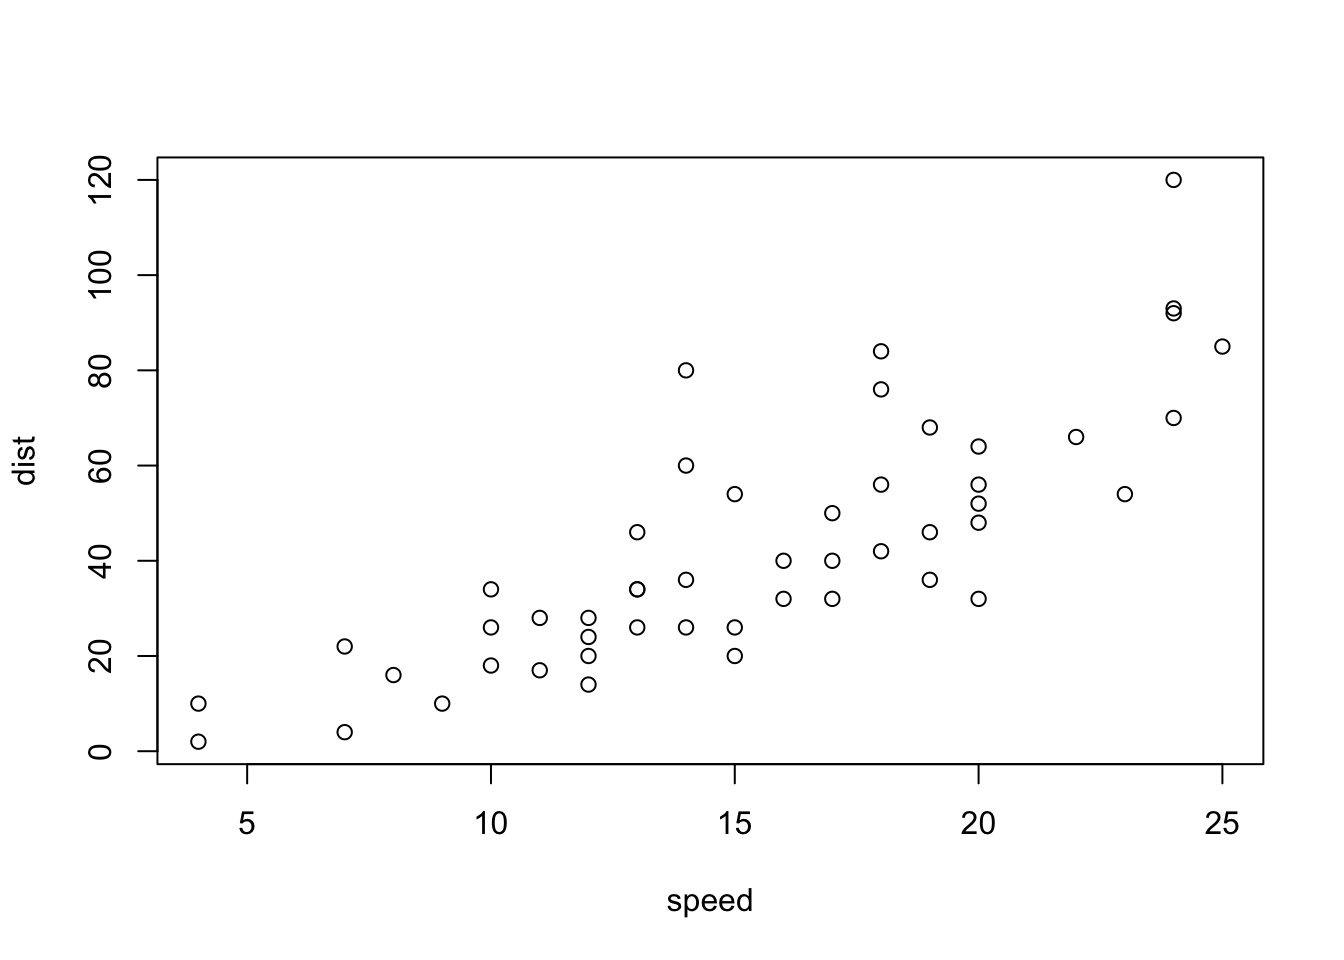
\includegraphics[width=5in]{863-UnsupervisedGenetics_files/figure-latex/unnamed-chunk-12-1}



\end{document}
